\section{Door task}
	\label{sub:door}

\subsection{Outline of the door task}
%
At the DRC Finals, the door task was specially important because without passing through it,
the robot wouldn't be able to perform the five remaining tasks
(valve, wall, surprise, debris or terrain, and stairs).
   
In general, we can divide the execution of the door task into the following phases:
%
\begin{enumerate}
	\item Walking to the front of the door.
	\item Grasping the door lever.
	\item Turning the lever and opening the door.
	\item Walking through the door.
\end{enumerate}
%

%In the DRC Finals, it was announced that the door will be 
%
%\begin{itemize}
%\item push open style,
%\item with lever type door lever, and
%\item without door closer.
%\end{itemize}

At the end of the second phase, the robot ends up in a standing configuration with a hand grasping
the door lever.
Let us call this the {\it open-door pose} as illustrated in \figurename~\ref{fig:door_approaching_config}.
In our approach, we determine a specific standing stance and a wrist attitude with respect to 
the door lever as shown in the figure.
In this way, the remaining phases 3) and 4) start from the same configuration;
thus we can use a pre-programmed sequence for operating the door and passing through it.
Even if we face variations of the door's geometry,
they can be handled by means of a minimum modifications.

\begin{figure}[t]
  \centering
  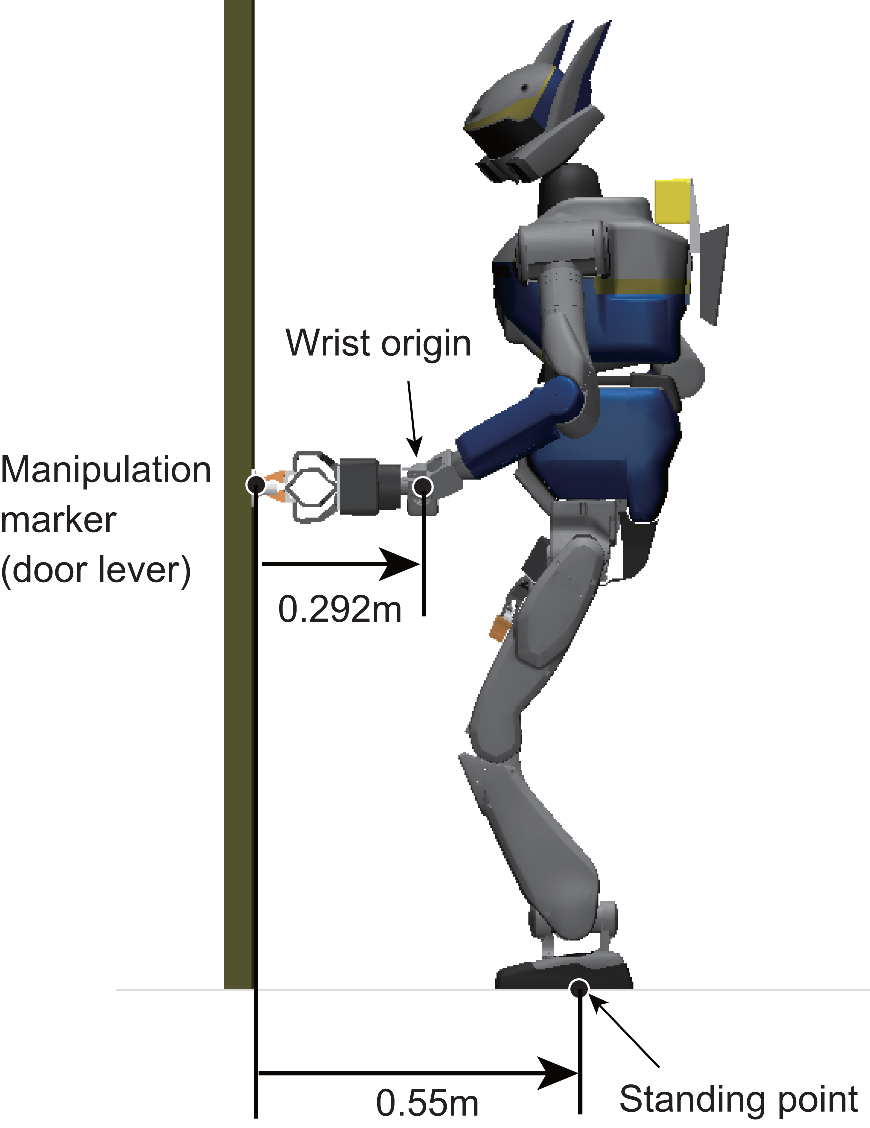
\includegraphics[width = 6.25cm]{img/door_approaching_config}
  \caption{Open-door pose}
  \label{fig:door_approaching_config}
\end{figure}

%From Step1 to Step2, we control our robot to realize the door approaching pose.
%To realize a reliable door passing, we pre-determined
%a robot pose grasping the door lever.
%Let us call it as {\it door approaching pose} which specifies the
%wrist point and the standing point with respect to the door lever

%The door lever operation (Step3) and the door passing through (Step4) always start
%from this fixed configuration. This means we can use a programmed sequence or its minimum
%modification at the door task.  

In the following subsections, we explain in detail phases 1) and 2); that is,
the way to control the robot to achieve the open-door pose by using sensor information
and teleoperation.
Phases 3) and 4) can be easily implemented. 
Especially at the DRC Finals, once the door had been opened wide enough, it ended up opening
completely by means of gravity and remaining open, since the door hinge was inclined 2.6 degrees
away from the vertical.
This helped the robots to walk through the door without worrying about any collision with
the opened door panel, which would eventually hit the robot by means of the action of the wind if the door hinge 
was vertical. 

\subsection{Walking to the front of the door}
%
To navigate the robot to the pose specified in \figurename~\ref{fig:door_approaching_config},
we used the point cloud data measured by the LRF. 
We took a two-step manual operation to identify the door orientation and the position of the
door lever as illustrated in \figurename~\ref{fig:door_manip_markers}.

First, the operator specifies a point on the left edge of the door panel
(\figurename~\ref{fig:door_manip_markers}(a) the `x' mark pointed by the arrow).
By applying the least square method to the portion of the point cloud located at the right of
the specified point, we can calculate the orientation of the door panel.
The result is shown by the {\it door marker}, a gray rectangle in
\figurename~\ref{fig:door_manip_markers}(b).
It covers a part of the door panel and we can interactively manipulate it on the point cloud GUI.
By adjusting the door marker, we can mask the points of the door panel and extract the points of
the door lever as shown in \figurename~\ref{fig:door_manip_markers}(c).
%Since the door lever is relatively small with respect to the point cloud resolution,
%it contains only 10 to 20 points which makes conventional model fitting very difficult.
%Thanks to the robustness of the human perception, 
In this way, we can confidently mark the rotation center of the lever (pointed by the arrow).
\figurename~\ref{fig:door_manip_markers}(d) shows the manipulation marker for the door lever
placed on the point cloud.
Its position and orientation are used to navigate the robot to the desired pose for opening
the door.

\begin{figure}[t]
  \centering
  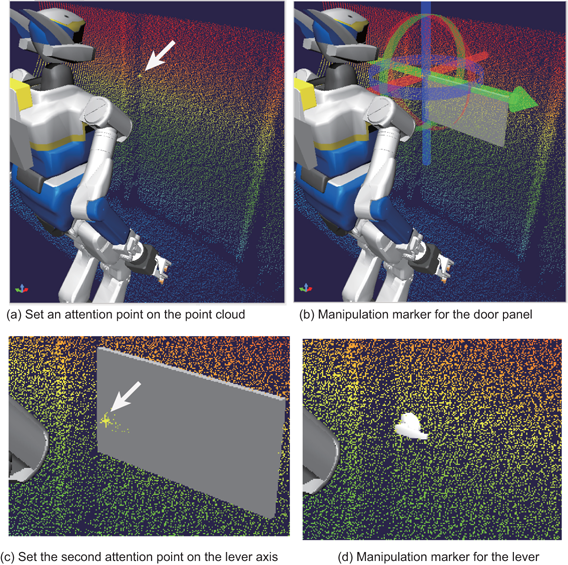
\includegraphics[width = 8cm]{img/door_manipulation_markers}
  \caption{Detection of the door lever in the control window}
  \label{fig:door_manip_markers}
\end{figure}

\subsection{Grasping the door lever}
%
Now the robot is standing on a good place to grasp the door lever.
%By the method of previous subsection, we can expect our robot is standing in front of the door
%aligned to its surface normal with desired distance.
Instead of grasping the door lever directly, we move the robot hand to an {\it approach point},
which is placed at a certain distance (0.13m) from the lever. 
This is because the hand position may not be accurate enough due to the LRF measurement noise,
calibration error, and slip occurring while walking.

Figure \ref{fig:door_lever_grasp}(a) shows the robot at the open-door pose and its hand at the
approach point (right window) in Choreonoid simulator.
The left window shows the simulated view of the left hand camera.
Both images show that the left hand is not appropriate to grasp the door lever (too left).
Note that during the real robot control, only the camera view is available. 

The operator can manually adjust the hand position by using some GUI buttons: 
{\it Left}, {\it Right}, {\it Down}, and {\it Up}, as seen in the left bottom window.
In this case, the operator can adjust the hand position by hitting {\it Right} button
several times.
Figure \ref{fig:door_lever_grasp}(b) shows the adjusted hand position to grasp the lever.

Figure \ref{fig:door_lever_grasp}(c) shows the final state getting a good grasp of the door lever.
From this moment, the point cloud based manipulation marker is no longer used.
For example, the rotation center of the lever is determined using the hand position calculated from
the internal sensors (joint encoders and posture sensors). 
%By hitting the button 'OK', the robot move the left hand forward until it contacts the door surface (we specified a sleshold of 5N to detect the contact).  The hand is in contact with appropriate position to grasp the door lever in \figurename~\ref{fig:door_lever_grasp}(c).
%
\begin{figure}[t]
  \centering
  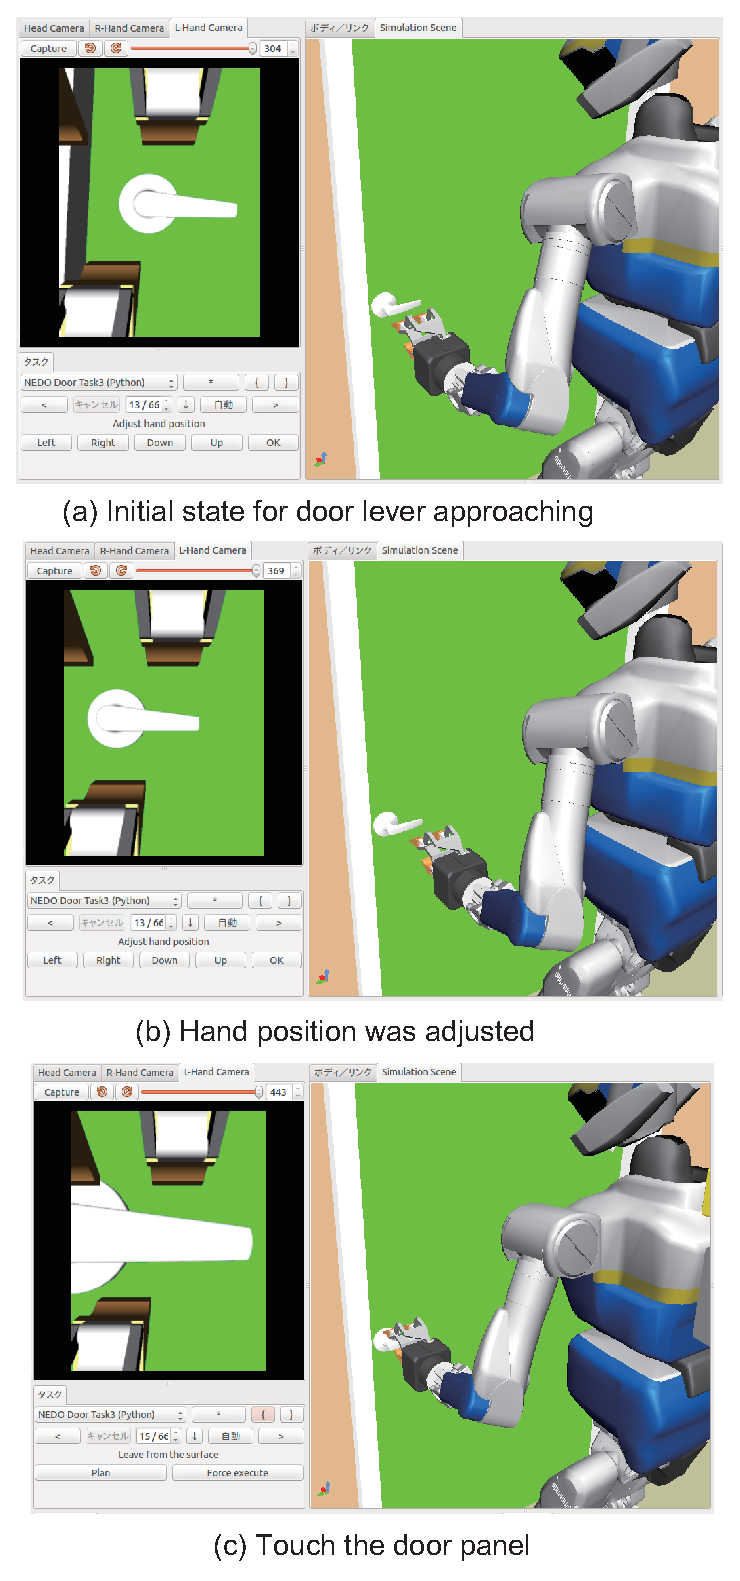
\includegraphics[width = 7.5cm]{img/approach_door_lever}
  \caption{Approach for grasping the door lever}
  \label{fig:door_lever_grasp}
\end{figure}

%\begin{figure}[t]
%  \centering
%  \includegraphics[width = 7.5cm]{img/open_the_door}
%  \caption{Door opening}
%  \label{fig:door_opening}
%\end{figure}

\subsection{Result at the DRC Finals}
%
At the DRC Finals 2015, HRP-2Kai cleared the door task at the rehearsal on June 4 and during
the challenge on June 6.
\figurename~\ref{fig:drc_door_aist_day2} shows the robot (a) while scanning with the LRF to
obtain a point cloud, (b) walking to the the open-door pose, (c) grasping the door lever,
and (d) opening the door successfully.
The robot spent 5 minutes and 21 seconds from the LRF scanning to fully pass the door.
%
\begin{figure}[t]
  \centering
  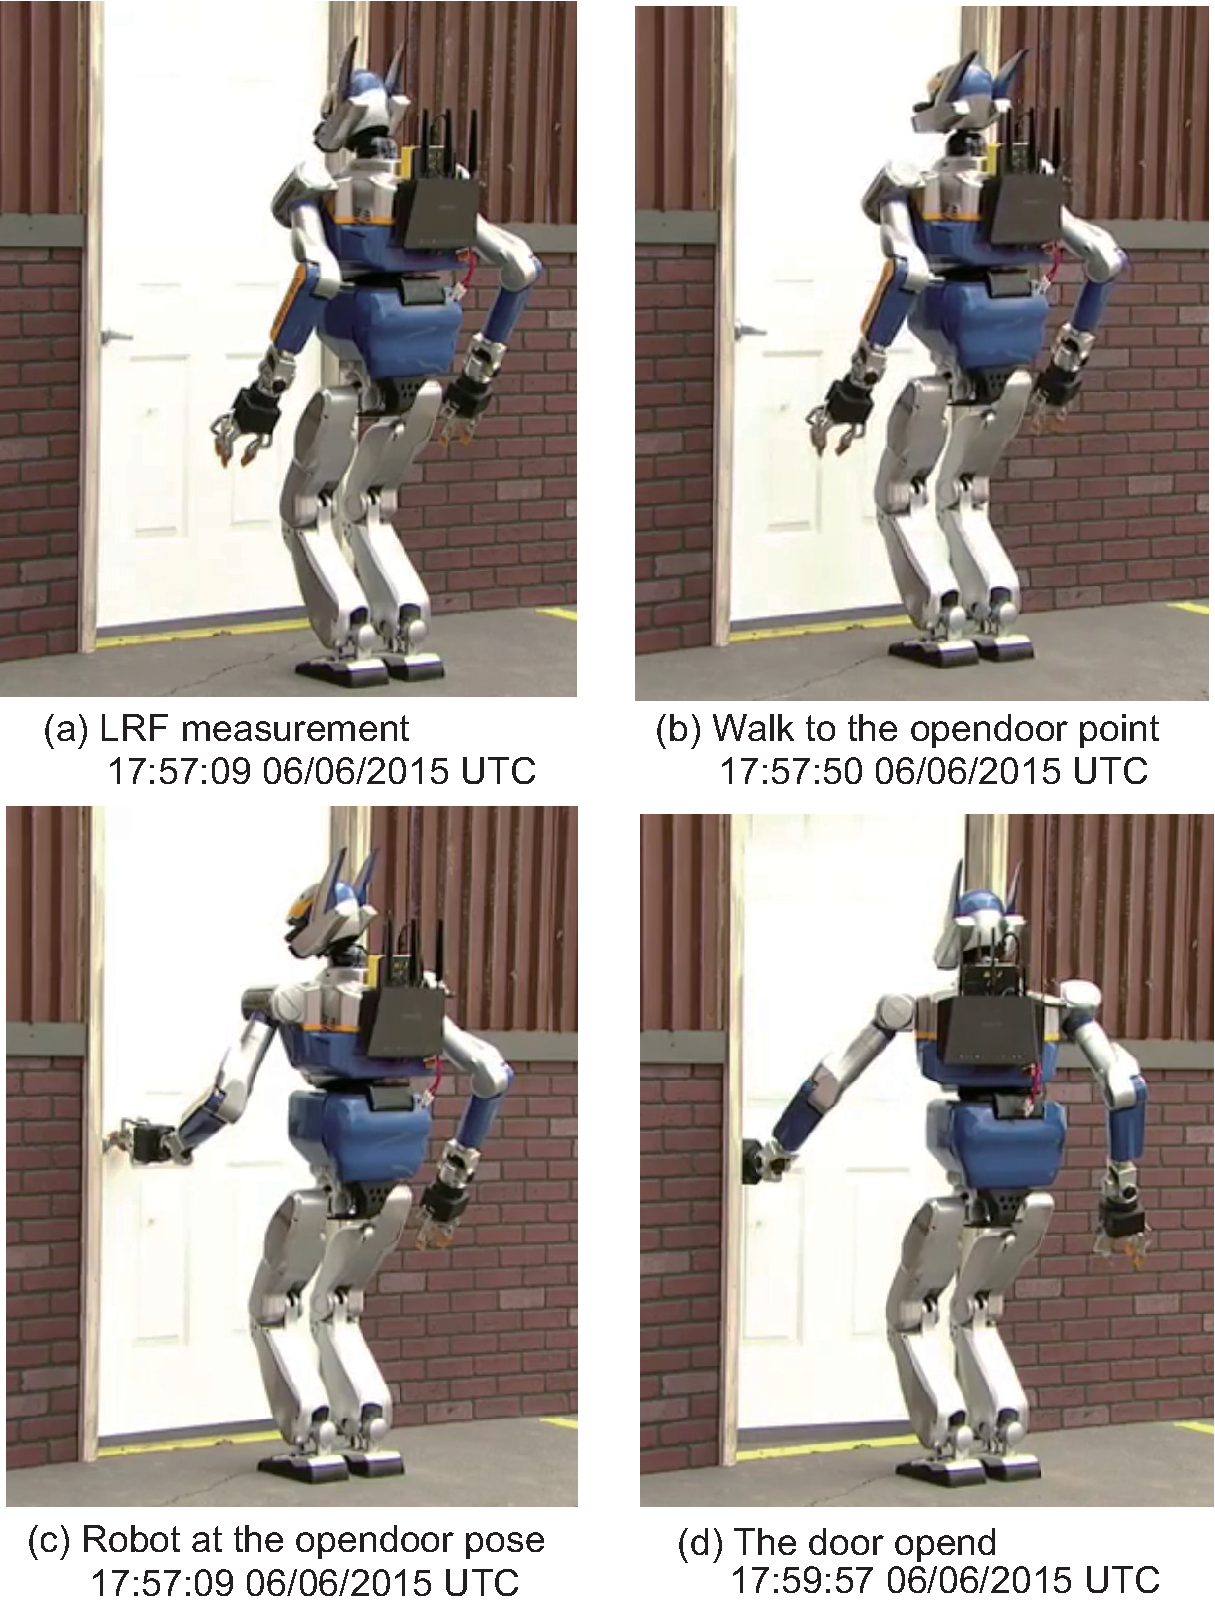
\includegraphics[width = 7.5cm]{img/drc_door_aist_day2}
  \caption{Door task at DRC Finals on June 6~\cite{DARPA}}
  \label{fig:drc_door_aist_day2}
\end{figure}

During the challenge on June 5, HRP-2Kai failed to operate the door lever at first,
requiring a second attempt to grasp it again, which was done by manual teleoperation.
During this operation, we experienced a low level control system crash, and the robot
fell down (\figurename~\ref{fig:drc_door_aist_day1}).
Since the computer stopped working and the hardware was damaged, we had to abort the
challenge for that day. 
%
\begin{figure}[t]
  \centering
  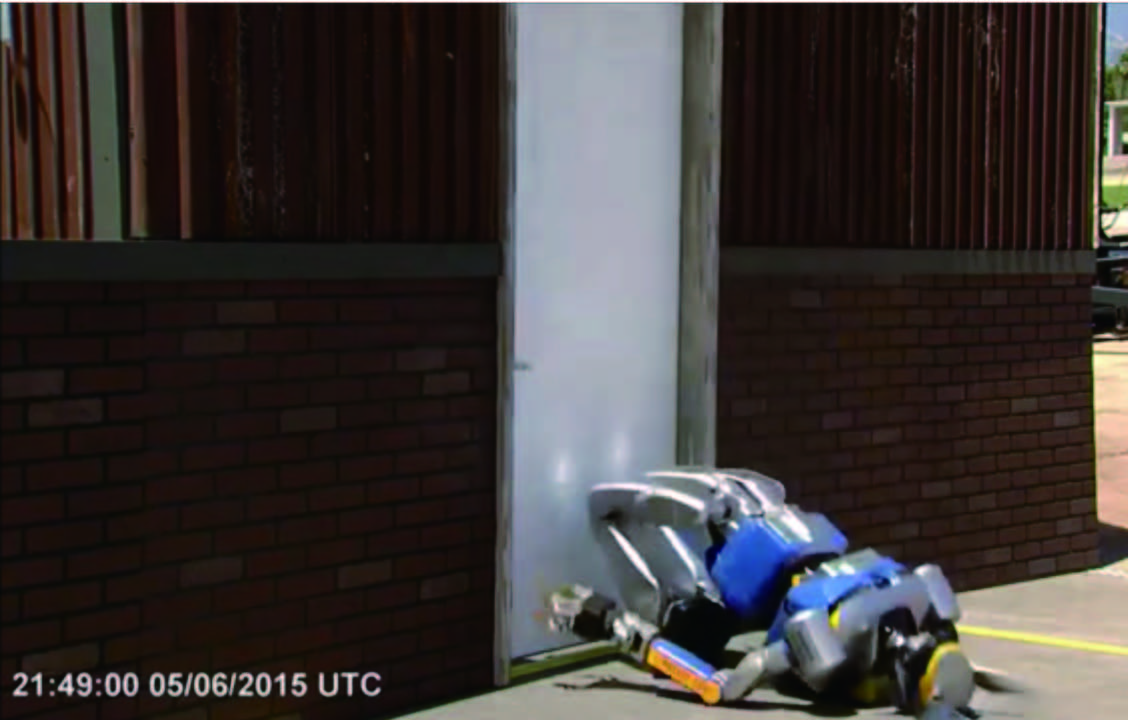
\includegraphics[width = 7.5cm]{img/drc_door_aist_day1}
  \caption{Control system crash at DRC Finals on June 5~\cite{DARPA}}
  \label{fig:drc_door_aist_day1}
\end{figure}

The robot failed to operate the lever because the doors in DRC Finals had different
latch properties, as shown in Table~\ref{tbl:door_latch}.
On day 1, we hard-corded the latch rotation angle as 30 degrees,
which worked at the rehearsal.
Of course, such implementation is not acceptable for the actual disaster response robots.
%
\begin{table}[htb]
\caption{Door latch properties at DRC finals} \label{tbl:door_latch}
\begin{tabular}{lclc}
\hline
Course & Latch release angle & Date & Door task result  \\ 
\hline
Green & 30 deg & June 4 (rehearsal) & Success  \\
Yellow & 70 deg & June 5 (day 1) & Fail \\
Blue &  50 deg & June 6 (day 2)  & Success \\
\hline
\end{tabular}
\end{table}

